\documentclass{ximera}
\title{Cylindrical Coordinates}
\begin{document}
\begin{abstract}
\end{abstract}
\maketitle

In this activity, we introduce cylindrical coordinates, a new coordinate system on $\mathbb{R}^3$.

\section{Cylindrical Coordinates}

We've seen how points in $\mathbb{R}^2$ can be written using polar coordinates. Polar coordinates can be useful for describing shapes that are difficult to describe in Cartesian coordinates.

We'd now like to extend this idea to $\mathbb{R}^3$, using a coordinate system called \emph{cylindrical coordinates}. Like polar coordinates, cylindrical coordinates will be useful for describing shapes in $\mathbb{R}^3$ that are difficult to describe using Cartesian coordinates. Later in the course, we will also see how cylindrical coordinates can be useful in multivariable Calculus, when differentiating or integrating in Cartesian coordinates is difficult or impossible.

Cylindrical coordinates really are just a simple extension of polar coordinates. For points in the $xy$-plane, we describe them using $r$ and $\theta$, where $r$ is the distance from the origin and $\theta$ is the angle with the positive $x$-axis. We then tack on a $z$-coordinate, the exact same as the $z$-coordinate in Cartesian coordinates, which tells us the vertical displacement of the point.

\begin{image}
\begin{tikzpicture}

\draw[<->] (-2.5,0) -- (2.5,0);
\draw[<->] (0,-2.5) -- (0,2.5);
\draw[<->] (-2,-1.5) -- (2,1.5);

\node at (2.5, -.25) {$y$};
\node at (-.3, 2.5) {$z$};
\node at (-2, -1.75) {$x$};

\node[draw, circle, thick, fill=black, minimum size=1mm, inner sep=0] at (1,1) {};

\draw[dashed] (1,1) -- (1,-3/4);
\draw[dashed] (1,-3/4) -- (0,0);
\draw (-0.2,-0.15) arc (250:295:.5);

\node at (1, 1.24) {$(r,\theta, z)$};
\node at (1.1, .25) {$z$};
\node at (.6,-.3) {$r$};
\node at (-.1,-.35) {$\theta$};

\end{tikzpicture}
\end{image}

\begin{example}
Let's look at what happens in cylindral coordinates when we set each of the coordinates $r,\theta,z$ to be constant.

That is, we'll begin by examining the set of points $(C,\theta, z)$, where $C$ is a constant. We have that $r=C$ is constant, which means that the distance between any such point and the $z$ axis is constant, $C$. Also, $\theta$ and $z$ can be anything. This will give us the cylinder of radius $C$, centered at the $z$-axis.

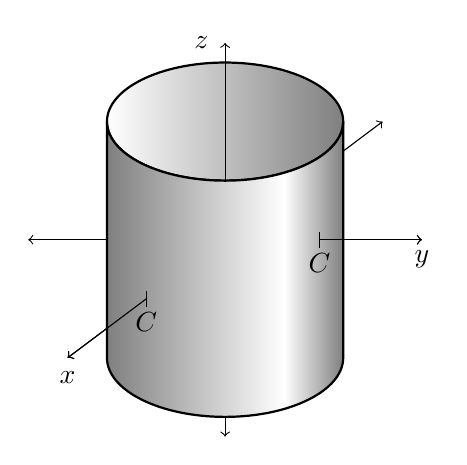
\begin{tikzpicture}

\coordinate (ll) at (-1.5,-1.5);
   \coordinate (lr) at (1.5,-1.5);
   \coordinate (ul) at (-1.5,1.5);
   \coordinate (ur) at (1.5,1.5);

\draw [thick, shade, shading angle=270] (ul) arc (-180:180:1.5cm and .75cm);

\draw[<->] (-2.5,0) -- (2.5,0);
\draw[<->] (0,-2.5) -- (0,2.5);
\draw[<->] (-2,-1.5) -- (2,1.5);

\node at (2.5, -.25) {$y$};
\node at (-.3, 2.5) {$z$};
\node at (-2, -1.75) {$x$};


   \shade [shading angle=90] (ll) arc (-180:-60:1.5cm and .75cm) -- +(0,3) arc (-60:-180:1.5cm and .75cm) -- cycle;
   
   \shade [shading angle=270] (lr) arc (0:-60:1.5cm and .75cm) -- +(0,3) arc (-60:0:1.5cm and .75cm) -- cycle;
   
   \draw [thick] (ll) arc (-180:0:1.5cm and .75cm) -- (ur) arc (0:-180:1.5cm and .75cm) -- cycle;
   
\draw[->] (-1,-0.75) -- (-2,-1.5);
\draw[->] (1.2,0) -- (2.5,0);

\draw (1.2,-.1) -- (1.2, .1);
\node at (1.2, -.3) {$C$};

\draw (-1,-.65) -- (-1, -.85);
\node at (-1, -1.05) {$C$};
   
\end{tikzpicture}
\end{example}

$\theta = C$

$z = C$

\section{Converting between Cartesian and cylindrical coordinates}

Perhaps not surprisingly, converting between Cartesian coordinates and cylindrical coordinates is very similar to how we converted between Cartesian coordinates and polar coordinates. That is, we can use the equations:
\begin{align*}
x &= r\cos\theta, \\
y &= r\sin\theta, \\
z &= z.
\end{align*}
It can also be very useful to use the fact that $x^2 + y^2 = r^2$.


\end{document}